\section{Introductory concepts}

%%%%%%%%%%%%%%%%%%%%%%%%%%%
% *** FIRST SUB-SECTION ***
%%%%%%%%%%%%%%%%%%%%%%%%%%%
\subsection{Hash functions}
A hash function is a fuction that maps an arbitrary long input string to a fixed
length output string. Let $h$ refer to an hash function of length $n$:

\[
  h\colon \{0,1\}^* \to \{0,1\}^n
\]

$m$ is usually called ``the message'', while $d$ is usually called ``the digest``
and it can be seen as a compact representation of m. The length of $d$ is the

Hash functions are usually used to provide data integrity and they're also used to
construct other cryptographic primitives such as MACs and digital signatures.

\subsubsection{Desired properties}
An hash function should ideally meet these properties:
\begin{itemize}
  \item \textbf{Computational efficiency}: given m, it must be easy to compute ${d=h(m)}$
  \item \textbf{Preimage resistance} (also called \textbf{one-way property}):
  given ${d=h(m)}$, it must be computationally infeasible computing $m$ ($m$ is the
  preimage)
  \item \textbf{Weak collision resistance} (also called
  \textbf{2\textsuperscript{nd} preimage resistance}): given $m_1$ and ${d_1=h(m_1)}$,
  it must be computationally infeasible finding a $m_2 \neq m_1$ so that ${h(m_2)=d_1}$
  \item \textbf{Strong collision resistance}: it must be computationally infeasible
  finding pairs of distinct and colliding messages. Two messages $m_1\neq m_2$
  collide when ${h(m_1)=h(m_2)}$.
  \item \textbf{Avalanche effect}: changing a single bit of $m$ should cause every
  bit of ${d=h(m)}$ to change with probability ${P=0.5}$
\end{itemize}

\subsubsection{Examples of hash functions}
\begin{itemize}
  \item \textbf{MD5}: published in 1991, it's a 128-bit hash function that was
  used for file integrity checks. Today it's considered insecure and it shouldn't
  be used anymore.
  \item \textbf{Secure Hash algorithm 1 (SHA-1)}: 160-bit hash function that was
  used in SSL and TLS implementations. Today is considered insecure and it's
  deprecated.
  \item \textbf{SHA-2}: family of SHA functions which includes SHA-256, SHA-384
  and SHA-512. SHA-256 is currently used in several parts of the Bitcoin network.
  \item \textbf{SHA-3}: latest family of SHA functions, it is a NIST-standardized
  version of Keccak, which uses a new approach called ``sponge construction''
  instead of the Merkle-Damgard transformation previously used. This family
  includes SHA3-256, SHA3-384 and SHA3-512.
\end{itemize}












\subsubsection{Design of SHA-256} SHA-256 works on 512-bits blocks and the input
message size has to be $< 2^{64}$bit. The outpus size is 256 bits. The algorithm
can be divided in two phases: pre-processing and hash computation.

\paragraph{Pre-processing}
\begin{enumerate}
  \item Padding of the message so that its length is a multiple of 512 bits.
  \item Parsing the message into N blocks of 512 bits $M(0), M(1), \dots, M(N)$.
  The first 32 bits of a block $i$ are denoted $M_0(i)$, the next 32 bits
  are $M_1(i)$ and so on up to $M_{15}(i)$.
  \item Setup of the initial has value $H(0)$, which is a sequence of eight 32-bits
  words obtained by taking the first 32-bits of the fractional parts of the
  square roots of the first eight prime numbers.
\end{enumerate}


\paragraph{Hash computation} The blocks of the message are processed one at a
time, beginning with $H(0)$, as follows:
\[ H(i) = H(i-1) + C_{M(i)}(H(i-1)) \]
where $+$ is the $\bmod 32$ addition and $C$ is the SHA-256 compression function,
which is shown if figure \ref{fig:sha256-compress-function} and it's basically
a block cipher which uses the message block $M(i)$ as key.

$H(N)$ is the hash of the message $M$.

\begin{figure}[!htb]
	\centering
	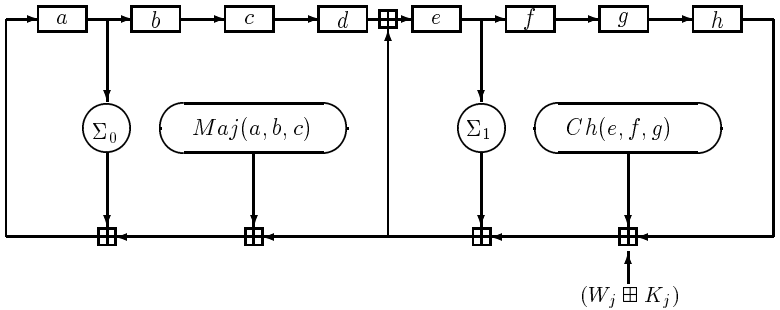
\includegraphics[width=1\linewidth]{img/sha-256-round.png}
	\caption{A round of the SHA-256 compress function $C$. The symbol $\boxplus$
  denotes the $\bmod 32$ addition, $Maj(X, Y, Z)=(X \cap Y) \oplus (X \cap Z) \oplus (Y \cap Z)$,
  $Ch(X,Y,Z)=	(X \cap Y) \oplus (!X \cap Z)$, $W_j$ and $K_j$ and round constants
  and $\sum_0$ and $\sum_1$ perform bitwise rotation.}
	\label{fig:sha256-compress-function}
\end{figure}

















\subsubsection{Message Authentication Codes (MACs)}
A MAC is an hash function which uses a key and which can therefore be used to
provide both integrity and authentication (proof of origin). Authentication is
based on a key pre-shared between the sender and the receiver. The receiver can
verify both integrity and authentication of a message by computing the MAC function
of the message and comparing it with the one received from the sender: if they are the
same then integrity and authentication are confirmed (note that it is assumed that
only the sender and the receiver know the key).

MAC functions can be constructed using block ciphers or hash functions:
\begin{itemize}
  \item in the first approach, block ciphers are used in the Cipher block chaining mode (CBC mode):
  the MAC of a message will be the output of the last round of the CBC operation.
  The length of MAC, in this case, is the same as the block length of the block cipher
  used to generate it.
  \item In the second approach, they key is hashed with the message using a certain
  construction scheme. The most simple ones are \emph{suffix-only} and
  \emph{prefix-only}, which however are weak and vulnerable:
  \begin{itemize}
    \item suffix-only: ${d=MAC_k(m)=h(m|k)}$, where $h$ is an hash function
    \item prefix-only: ${d=MAC_k(m)=h(k|m)}$, where $h$ is an hash function
  \end{itemize}
\end{itemize}





\subsection{Digital signature}
Digital signatures are used to associate a message with the entity from which the
message has been originated. They provide the same service as MACs (authentication
and non-repudiation) plus the non-repudiation.

Digital signature is based on public key cryptography: Alice can sign a message
by encrypting it using its private key. Usually, however, for efficiency and security
reasons, Alice doesn't encrypt the message but its digest (hash of the message).
Figure \ref{fig:digital-signature} shows how a generical digital signature function
works.

An example of digital signature algorithms are RSA and ECDSA.

\begin{figure}[!htb]
	\centering
	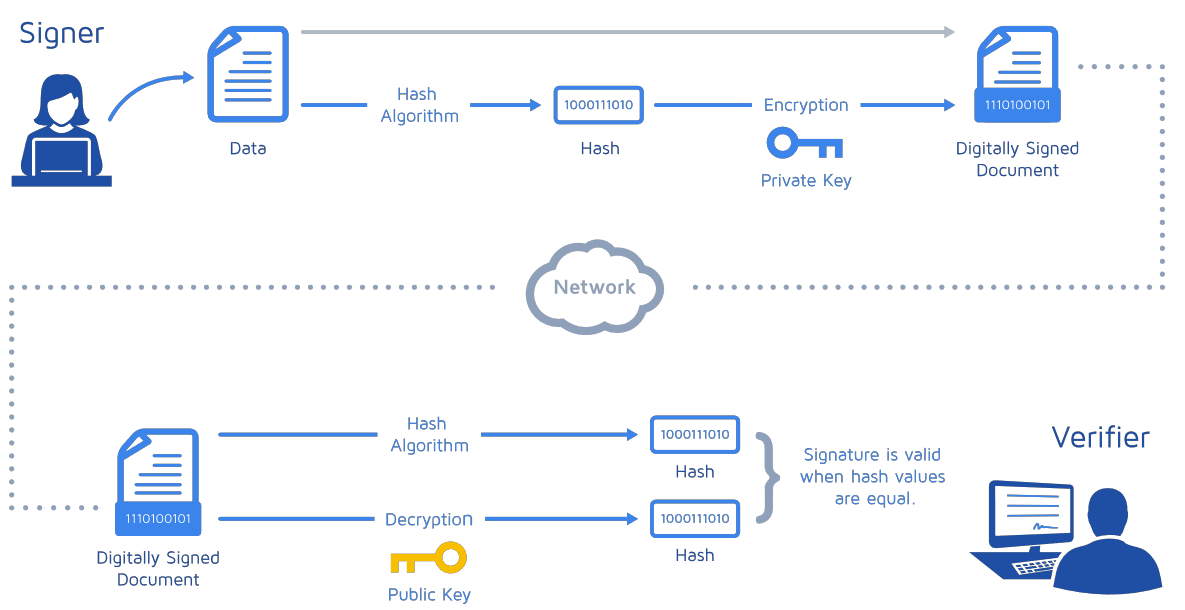
\includegraphics[width=1\linewidth]{img/digital-signature.png}
	\caption{digital signature signing and verification scheme}
	\label{fig:digital-signature}
\end{figure}





\subsection{Elliptic Curve Digital Signature Algorithm (ECDSA)}
ECDSA is a variant of the Digital Signature Algorithm (DSA) which uses elliptic
curve cryptography.

\subsubsection{Key pair generation}
\begin{enumerate}
  \item Define an elliptic curve $E$ with modulus $P$, coefficients $a$ and $b$ and a
  generator point $A$ that forms a cyclic group of order $p$, with $p$ prime
  \item Choose a random integer $d$ so that ${0 < d < q}$
  \item Compute the public key $B$ so that ${B = d  A}$
\end{enumerate}
The public key is the sextuple ${K_{pb} = (p,a,b,q,A,B)}$, while the private key
is the value of $d$ randomly chosen in Step 2: ${K_{pr} = d}$

\subsubsection{Signing a message}
\begin{enumerate}
  \item Choose an ephemeral key $K_e$, where ${0 < K_e < q}$.
  It should be ensured that $K_e$ is truly random and no two signatures have the same key
  because otherwise the private key can be calculated
  \item Compute ${R = K_e A}$
  \item Initialize a variable $r$ with the x coordinate value of the point $R$
  \item The signature on the message $m$ can be calculated as follow:
  \[{S=(h(m)+d r)K_e^{-1}\bmod q}\]
  where $h(m)$ is the hash of the message $m$. The signature is the pair ${(S,r)}$.
\end{enumerate}

\subsubsection{Signature verification}
A signature can be verified as follow:
\begin{enumerate}
  \item Compute ${w=S^{-1}\bmod q}$
  \item Compute ${u_1=w  h(m)\bmod q}$
  \item Compute ${u_2=w  r \bmod q}$
  \item Calculate the point ${P=u_1  A + u_2  B}$
  \item The signature ${(S,r)}$ is accepted as a valid signature only if:
   \[{X_P=r \bmod q}\]
   where $X_P$ is the x-coordinate of the point P calculated in Step 4
\end{enumerate}








%%%%%%%%%%%%%%%%%%%%%%%%%%%
% *** SECOND SUB-SECTION ***
%%%%%%%%%%%%%%%%%%%%%%%%%%%
\subsection{Blind signature} Blind signatures were introduced by David Chaum in
1982 \cite{chaum1982blind} and refer to a cryptographic primitive that allows an
entity to digitally sign a message without knowing or being able to read the
message that it signs. The following analogy introduced by Chaum himself clearly
explains what blind signatures are:

``\emph{Assume an envelope with both a piece of paper (e.g. a contract) and carbon
paper inside it. The envelope is sealed and sent to the signer. The signer
cannot see what is inside the envelope without breaking the seal. The signer
signs the envelope, and thanks to the carbon paper, the contract inside the
envelope gets signed too. The signer returns the envelope to the sender, who
opens it and extracts the carbon-signed contract.}''

Blind signature can be implemented using different schemes. In this section it will be
briefly discussed the RSA scheme proposed by Chaum. Another scheme based on the
Diffie-Hellman problem will be discussed in section \ref{sec:enh-sign}.

\subsubsection{RSA signature scheme} In RSA the public parameters are $n=pq$ and
a chosen $e$ relatively prime to $\varphi(n)$, while the private parameters are
the primes $p,q$, $\varphi(n)$ and \mbox{$d=e^{-1}\bmod\varphi(n)$}. The signer private
key is $d$ and its public key is $e$.

The signer can sign a message $m$ by computing the signature $s$:
\[ s=m^d\bmod n \]
Anyone can verify the signature using the signer public key and verify if the message
is equal to the result of the computation below:
\[ s^e = m^{ed}\bmod n= m \bmod n \]

\subsubsection{RSA blind signature scheme}
\begin{enumerate}
  \item Generation of a blinding factor $b=r^{e}\bmod n$,
  with $r$ random number
  \item The message $m$ is blinded with the blinding factor $b$ previously
  calculated: $m_{*}=b\cdot m\bmod n$
  \item The blinded message $m_*$ is sent to the signer. The signer signs it by
  computing $s_*$:
  \[ s_*=m_*^d\bmod n = b^d\cdot m^d\bmod n = r^{e\cdot d}\cdot m^d \bmod n = r\cdot m^d \bmod n \]
  \item The user can divide $s_*$ by $r$ for retrieving $s=m^d\bmod n$, namely
  the RSA signature of the message $m$
\end{enumerate}











%%%%%%%%%%%%%%%%%%%%%%%%%%%
% *** THIRD SUB-SECTION ***
%%%%%%%%%%%%%%%%%%%%%%%%%%%
\subsection{Distributed systems}
\subsubsection{What is a distributed system}
Blockchain at its core is basically a distributed system, therefore it is essential
to understand distributed systems before understanding Blockchain.

A distributed system is a network that consists of autonomous nodes, connected
using a distribution middleware, which acts in a coordinated way (passing
messages to each other) in order to achieve a common outcome and that can be
seen by the user as a single logical platform.

A node is basically a computer that can be seen as an individual player inside
the distributed system and it can be honest, faulty or malicious. Nodes that
have an arbitrary behavior (which can be malicious) are called \emph{Byzantine nodes}.

\begin{figure}[!htb]
	\centering
	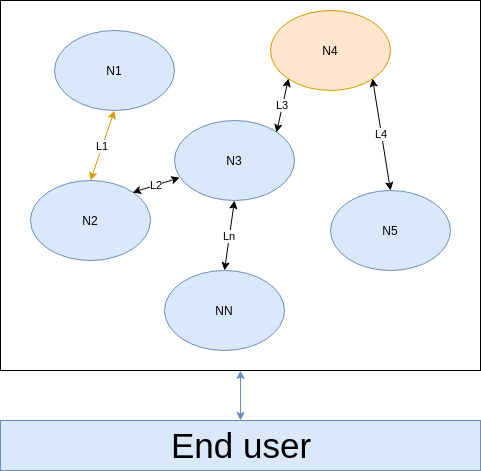
\includegraphics[width=0.6\linewidth]{img/distributed-system.png}
	\caption{design of a distributed system. N4 is a Byzantine node while L1 is a
  broken/slow network link}
	\label{fig:distributed-system}
\end{figure}

The main challenge in a distributed system is the fault tolerance: even if some
of the nodes fault or links break, the system should tolerate this and should
continue to work correctly. There are essentially two types of fault: a simple node
crash or the exhibition of malicious or inconsistent behavior arbitrarily. The
second case is the most difficult to deal with and it's called \emph{Byzantine
fault}. In order to achieve fault tolerance, replication is usually used.

Desired properties of a distributed system are the following:
\begin{itemize}
  \item \textbf{Consistency}: all the nodes have the same lates available copy of
  the data. It is usually achieved through consensus algorithms which ensure that
  all nodes have the same copy of the data
  \item \textbf{Availability}: the system is always working and responding to the
  input requests without any failures
  \item \textbf{Partition tolerance}: if a group of nodes fails the distributed
  system still continues to operate correctly
\end{itemize}
There is however a theorem, the \emph{CAP theorem}, which states (and proves)
that a distributed system cannot have all these three properties at the same time.
In particular, the theorem states that in the presence of a network partition (due
for example to a link failure) one has to choose between consistency and availability.



\subsubsection{Consensus}
Consensus is the process of agreement between untrusted nodes on a data value.
When the involved nodes are only two it's really easy to achieve consensus, while
in a distributed system with more than two nodes it is really hard (in this case
the process of achieving consensus is called \emph{distributed consensus}).
The data value agreed is the majority value, therefore the value proposed by
51\% of the nodes.

A consensus mechanism must meet these requirements:
\begin{itemize}
  \item \textbf{Agreement}: all the correct (non-faulty/malicious) nodes must agree on the same value
  \item \textbf{Termination}: the execution of the consensus process must come
  to an end and the nodes have to reach a decision
  \item \textbf{Validity}: the agreed value must have been proposed by at least
  one honest node
  \item \textbf{Fault tolerance}: the consensus algorithm must be able to run even
  in the presence of one or more Byzantine (faulty or malicious) nodes
  \item \textbf{Integrity}: the nodes make decisions only once in a single
  consensus cycle (in a single cycle a node cannot make the decision more than once).
\end{itemize}




\subsubsection{The Byzantine Generals Problem (BGP)}
The Byzantine Generals Problem (BGP) is a problem described by Leslie Lamport
\cite{lamport1982byzantine} in which a group of generals are surrounding a city
and they have to formulate a plan for attacking it (simplifying, they have to
decide whether to attack or retreat from the city).
Their only communication way is the messenger and they have to
agree on a common decision. The issue is that some of the generals may be
traitors trying to prevent the loyal generals from reaching an agreement by
communicating a misleading message. The generals need an algorithm to guarantee
that all the loyal generals agree on the same plan (attack or retreat) regardless
of what traitors generals do. Loyal generals will always do what the algorithm says they
should, while the traitors may do anything they wish.

As an analogy with distributed systems:
\begin{itemize}
  \item generals can be considered as nodes
  \item traitors can be considered Byzantine nodes
  \item the messenger can be seen as the channels of communication between the generals.
\end{itemize}

The problem can be see in term of generals-lieutenants: a General makes the
decision to attack or retreat, and must communicate the decision to his lieutenants.
Both the lieutenants and the general can be traitors: they cannot be relied upon
to properly communicate orders (traitor generals) and they may actively alter
messages in an attempt to subvert the process (traitor lieutenants).
\begin{figure}[!htb]
	\centering
	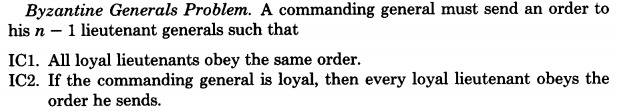
\includegraphics[width=1\linewidth]{img/byzantine-generals-problem.png}
	\caption{page 3 of the original Lamport's paper \cite{lamport1982byzantine}}
	\label{fig:byzantine-generals-problem}
\end{figure}

To solve this problem, Lamport proposed an algorithm for reaching consensus that
assumes that there are $m$ traitors and $3m$ actors. This implies that the
algorithm can reach consensus only if $2/3$ of the actors are honest: if the
traitors are more than $1/3$, consensus cannot be reached. The goal is
to make the majority of the lieutenants choose the same decision (not a specific one).
The original algorithm proposed by Lamport is shown in figure \ref{fig:lamport-byzantine-algorithm}.
\begin{figure}[!htb]
	\centering
	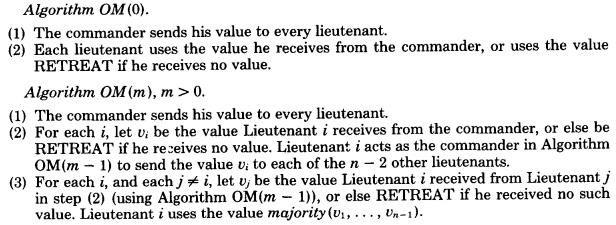
\includegraphics[width=1\linewidth]{img/lamport-byzantine-algorithm.png}
	\caption{Lamport's algorithm for reaching consensus}
	\label{fig:lamport-byzantine-algorithm}
\end{figure}



\subsubsection{Byzantine Fault Tolerance (BFT)}
A distributed system is said to be Byzantine Fault Tolerant when it tolerates a
the class of failures that belong to the Byzantine Generals’ Problem \cite{byzantine-konstantopoulos}.
In other words, a Byzantine Failure is a fault that presents different symptoms
to different observers and for this reason BFT is really difficult to achieve.

For example, a Byzantine Fault could be a node acting as a ``traitors'' and
generating arbitrary data during the process of reaching consensus.
